\subsection{Hivent List} % (fold)
\label{sub:hivent_list}

\subsubsection{General} % (fold)
\label{ssub:general_hl}
The central module to navigate \HG is the Hivent List. Here you can see Hivents with additional informations in one list ordered by date. Each Hivent has a name, a date and a location. She is located on the right edge of \HG under the search bar. They share the vertical amount.

\begin{figure}[H]
  \centering
  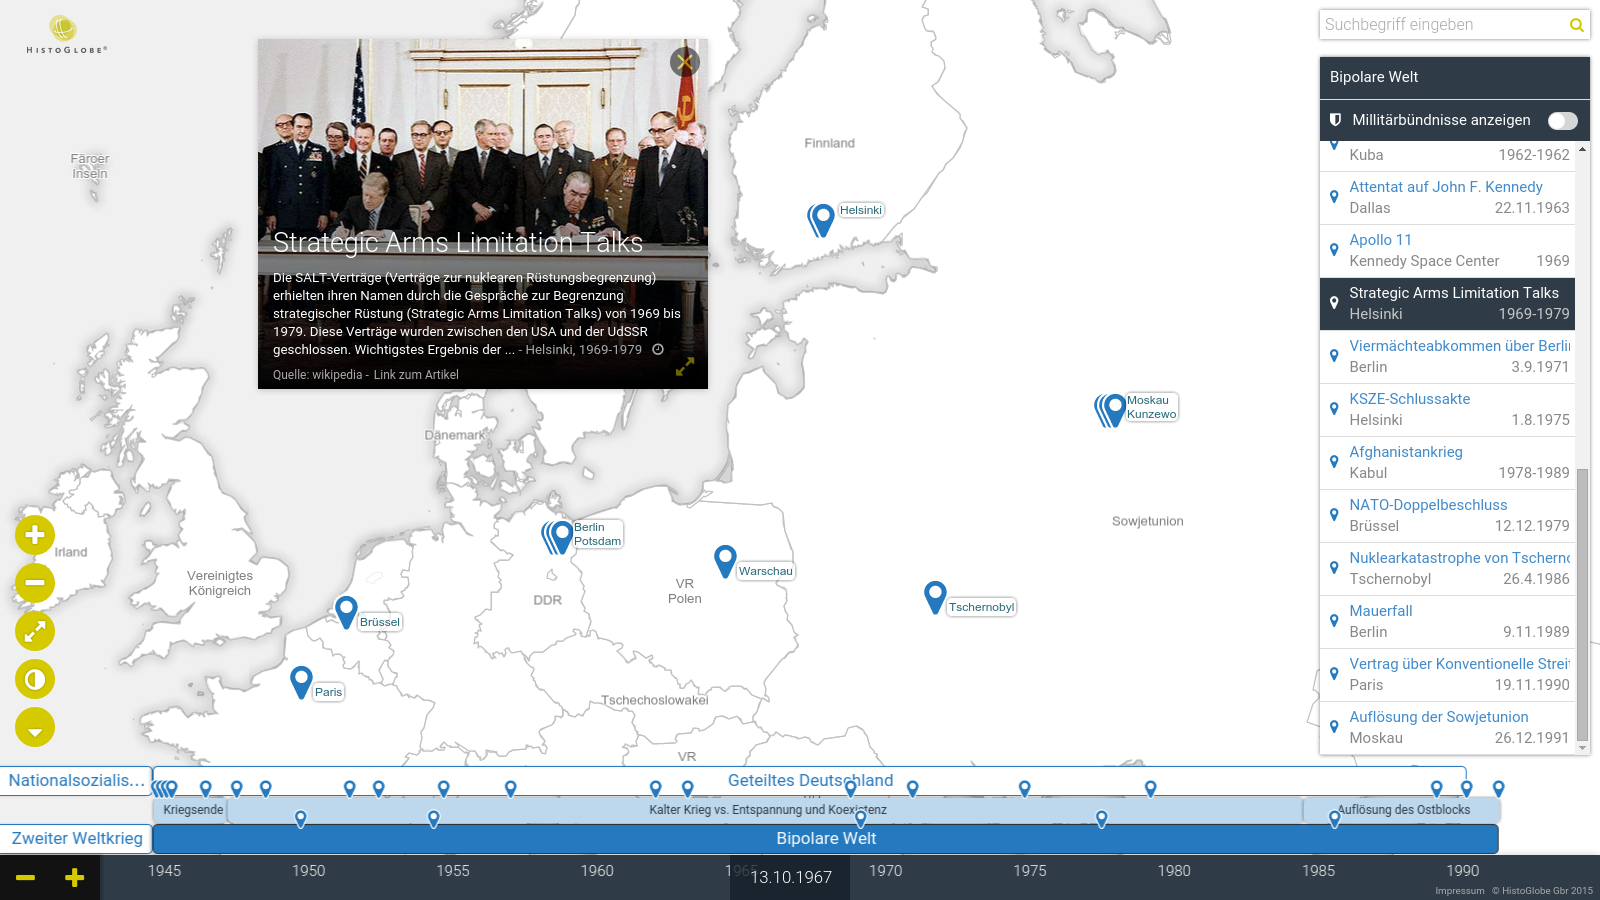
\includegraphics[width=0.9\textwidth]{graphics/final_ui.png}
  \caption{Hivent List}
\end{figure}

\subsubsection{Structure} % (fold)
\label{ssub:structure_hl}
The Hivent List module consists of title bar, an optional area and a list of Hivents. The title bar and the optional area have a fixed size and a fixed distance to the search bar. The list has a fixed distance to the Timeline and has the remaining amount available.

\begin{figure}[H]
  \centering
  \begin{minipage}{0.45\textwidth}
    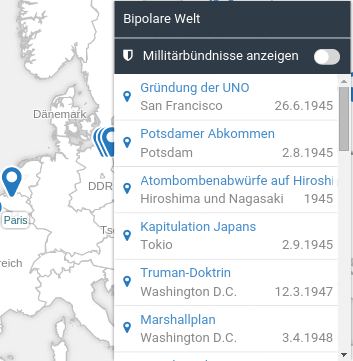
\includegraphics[width=0.95\textwidth]{graphics/bpa1.png}
  \end{minipage}
  \begin{minipage}{0.45\textwidth}
    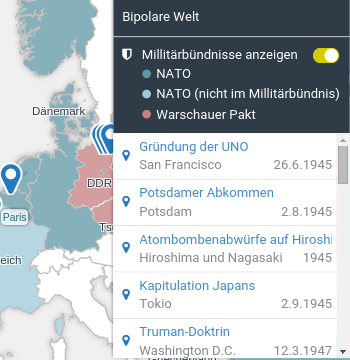
\includegraphics[width=0.95\textwidth]{graphics/bpa2.png}
  \end{minipage}
  \caption{Hivent List with and without active bipolar alliances}
  \label{fig:HL_options}
\end{figure}


\subsubsection{Behavior} % (fold)
\label{ssub:behaviour_hl}
The main function of the Hivent List is to give an overview to the user and than to enable and disable single Hivents. In the initial state of she is not available. 

For \textsc{activation} you have to click on one epoch. The second way is to search something and the Hivent List is initialized with the epoch of the searched Hivent.

To \textsc{deactivate} the Hivent list you can click on die active epoch in the Timeline.

The Search Bar is also an module to navigate through \HG. So they \textsc{share space} on the right side. If the Hivent List is active and you want to look for some other Hivent the searched results take the space of the Hivent List and only the title bar of the current epoch is displayed at the bottom.

\begin{figure}[H]
  \centering
  \begin{minipage}{0.45\textwidth}
    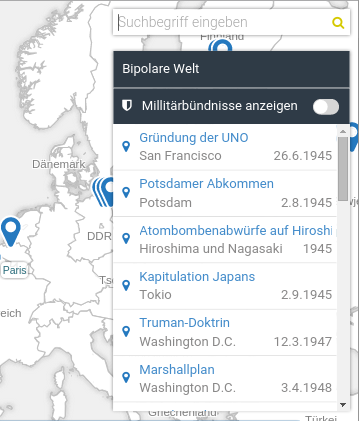
\includegraphics[width=0.95\textwidth]{graphics/hlsearch1.png}
  \end{minipage}
  \begin{minipage}{0.45\textwidth}
    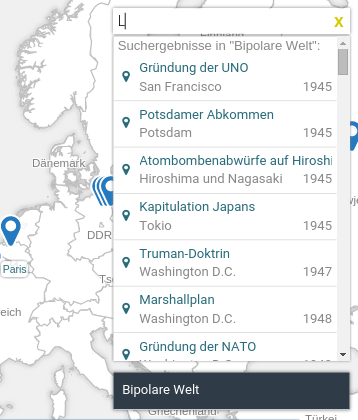
\includegraphics[width=0.95\textwidth]{graphics/hlsearch2.png}
  \end{minipage}
  \caption{Hivent List with and without search results}
\end{figure}

Between the title bar and a list of Hivents is the \textsc{epoch depending area} located. In our implementation only the "Bipolare Welt" has options as seen in Figure ~\ref{fig:HL_options}. Here you can switch the color of the countries on map in relationship to the membership to UNO and Warsaw Pact.

% subsection hivent_list (end)
